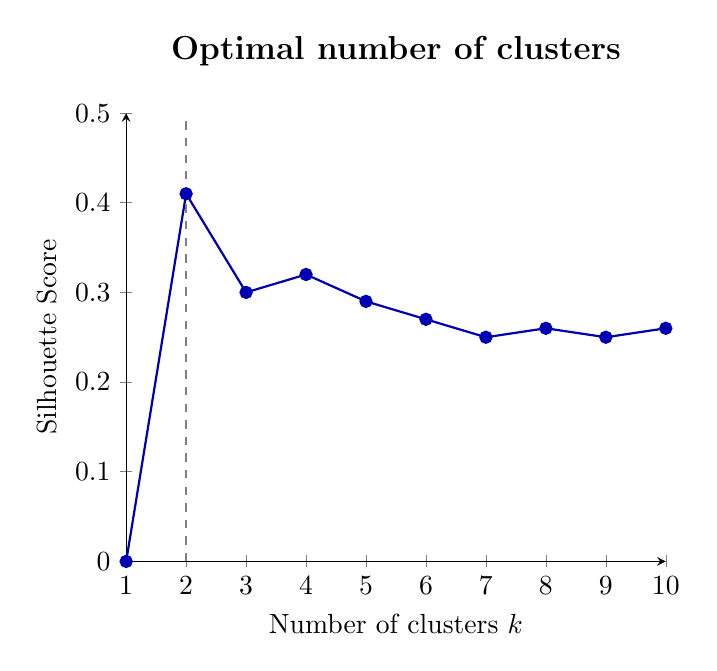
\begin{tikzpicture}
\begin{axis}[
    title={Optimal number of clusters},
    xlabel={Number of clusters $k$},
    ylabel={Silhouette Score},
    xmin=1, xmax=10,
    ymin=0, ymax=0.5,
    xtick={1,2,3,4,5,6,7,8,9,10},
    ytick={0,0.1,0.2,0.3,0.4,0.5},
    grid=none,
    axis lines=left,
    title style={at={(0.5,1.1)}, anchor=center, font=\bfseries\large},
]
% The Data Points
\addplot[color=blue!70!black,mark=*,thick,]
coordinates {
    (1,0.0) (2,0.41) (3,0.3) (4,0.32) (5,0.29) (6,0.27) (7,0.25) (8,0.26) (9,0.25) (10,0.26)
};
% The Vertical Dashed "Elbow" Line at k=4
\draw [dashed, thick, gray] (axis cs:2,0) -- (axis cs:2,0.5);
\end{axis}
\end{tikzpicture}
